\section{Configuración final}

Como he dicho en la sección de duración de la escena, es necesario animar manualmente desde el instante 0 hasta el instante 150, ambos inclusive. Además, todos los objetos deben incluir estos dos instantes porque si no se incluyen la animación inversa se realizaría antes de tiempo, provocando resultados no deseados, incluso dentro de los primeros 5 segundos.

\bigskip

Para que los otros 5 segundos se animen de manera inversa de forma automática, es necesario abrir el editor de curvas y darle al botón \textit{Parameter Curve Out-of-Range Types}. A continuación, hay que elegir la opción \textit{Ping Pong} tanto en el principio como en el final (aunque en el principio no es necesario, ya que no se va a ejecutar).

\begin{figure}[H]
   \centering
   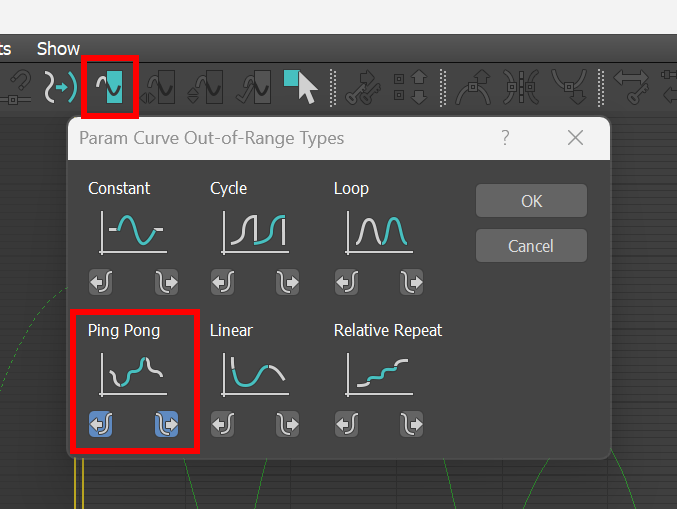
\includegraphics[width=0.5\textwidth]{imagenes/misc/ping-pong.png}
   \caption{Botones a los que hay que darle para poner la opción de ping-pong.}
\end{figure}

Cuando se selecciona esta opción, aparecerán en líneas discontinuas la curva que va a hacer en los instantes que no se han animado. Además, esto hay que hacerlo para cada objeto de la escena.

\bigskip

Por último, las curvas de todos los objetos animados, junto a su animación inversa son:

\begin{figure}[H]
   \centering
   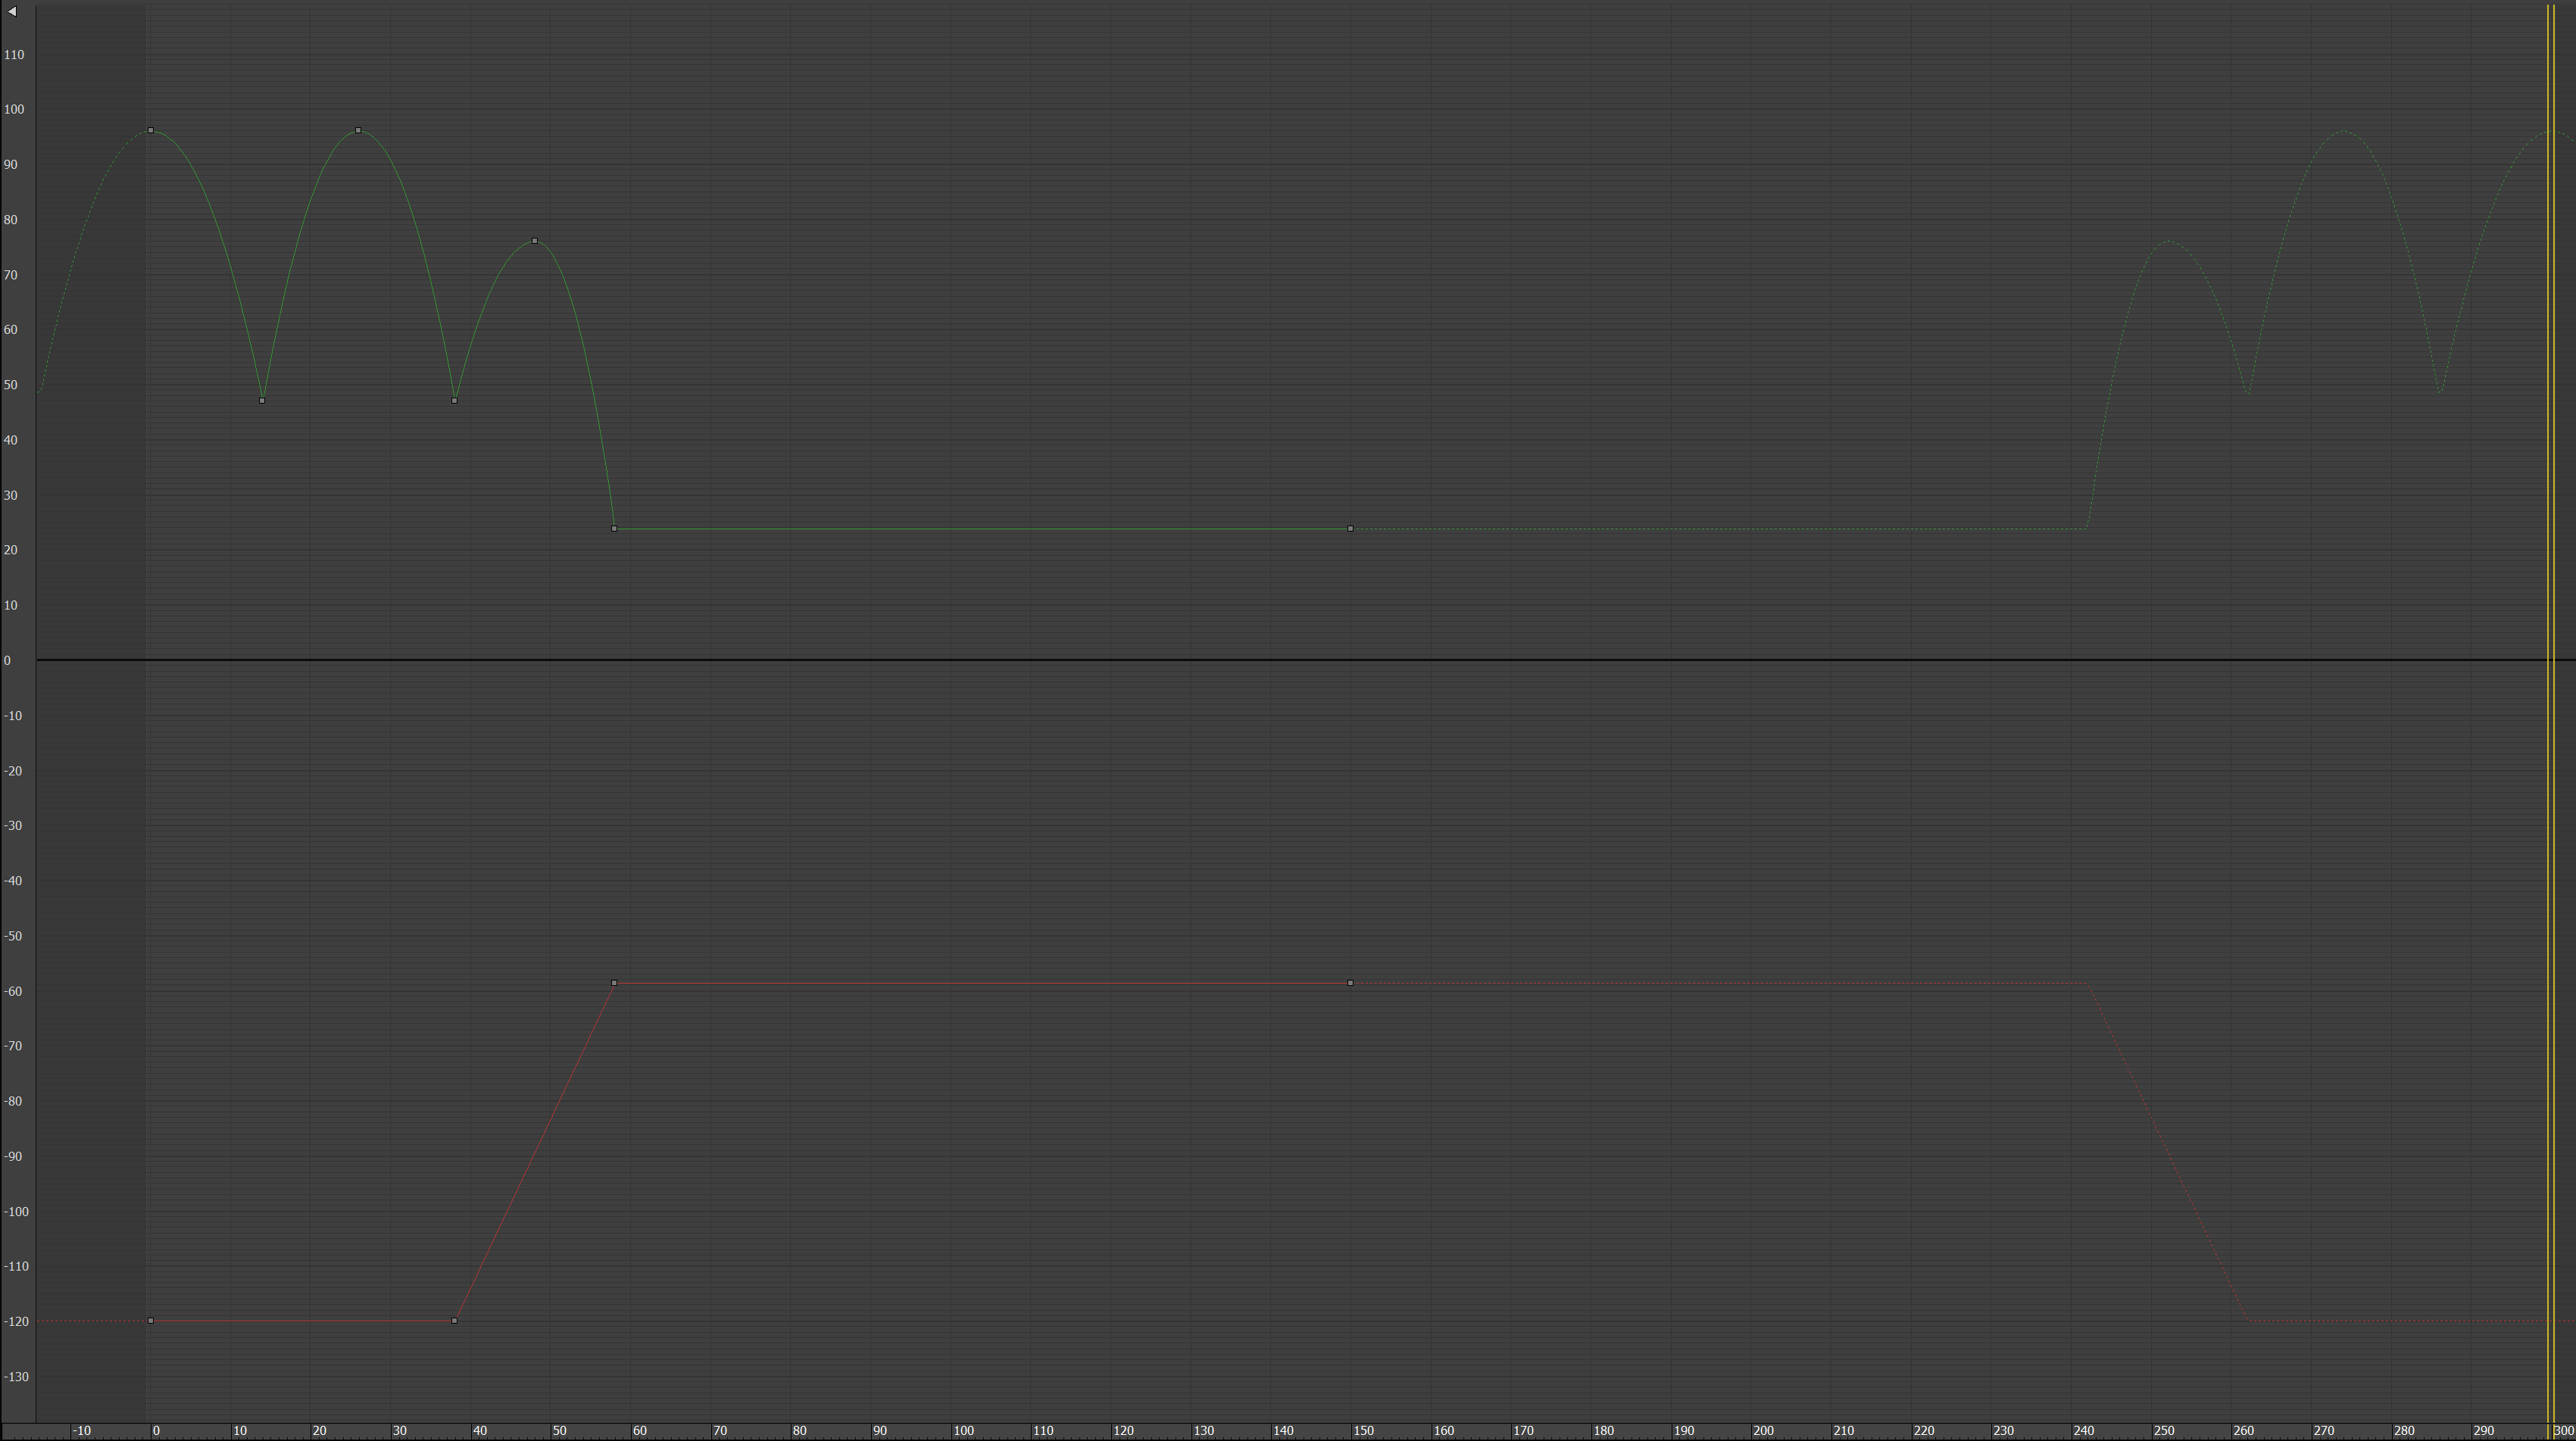
\includegraphics[width=0.7\textwidth]{imagenes/curvas finales/PL.png}
   \caption{Curva, junto a su inversa, de la pelota de la izquierda.}
\end{figure}

\begin{figure}[H]
   \centering
   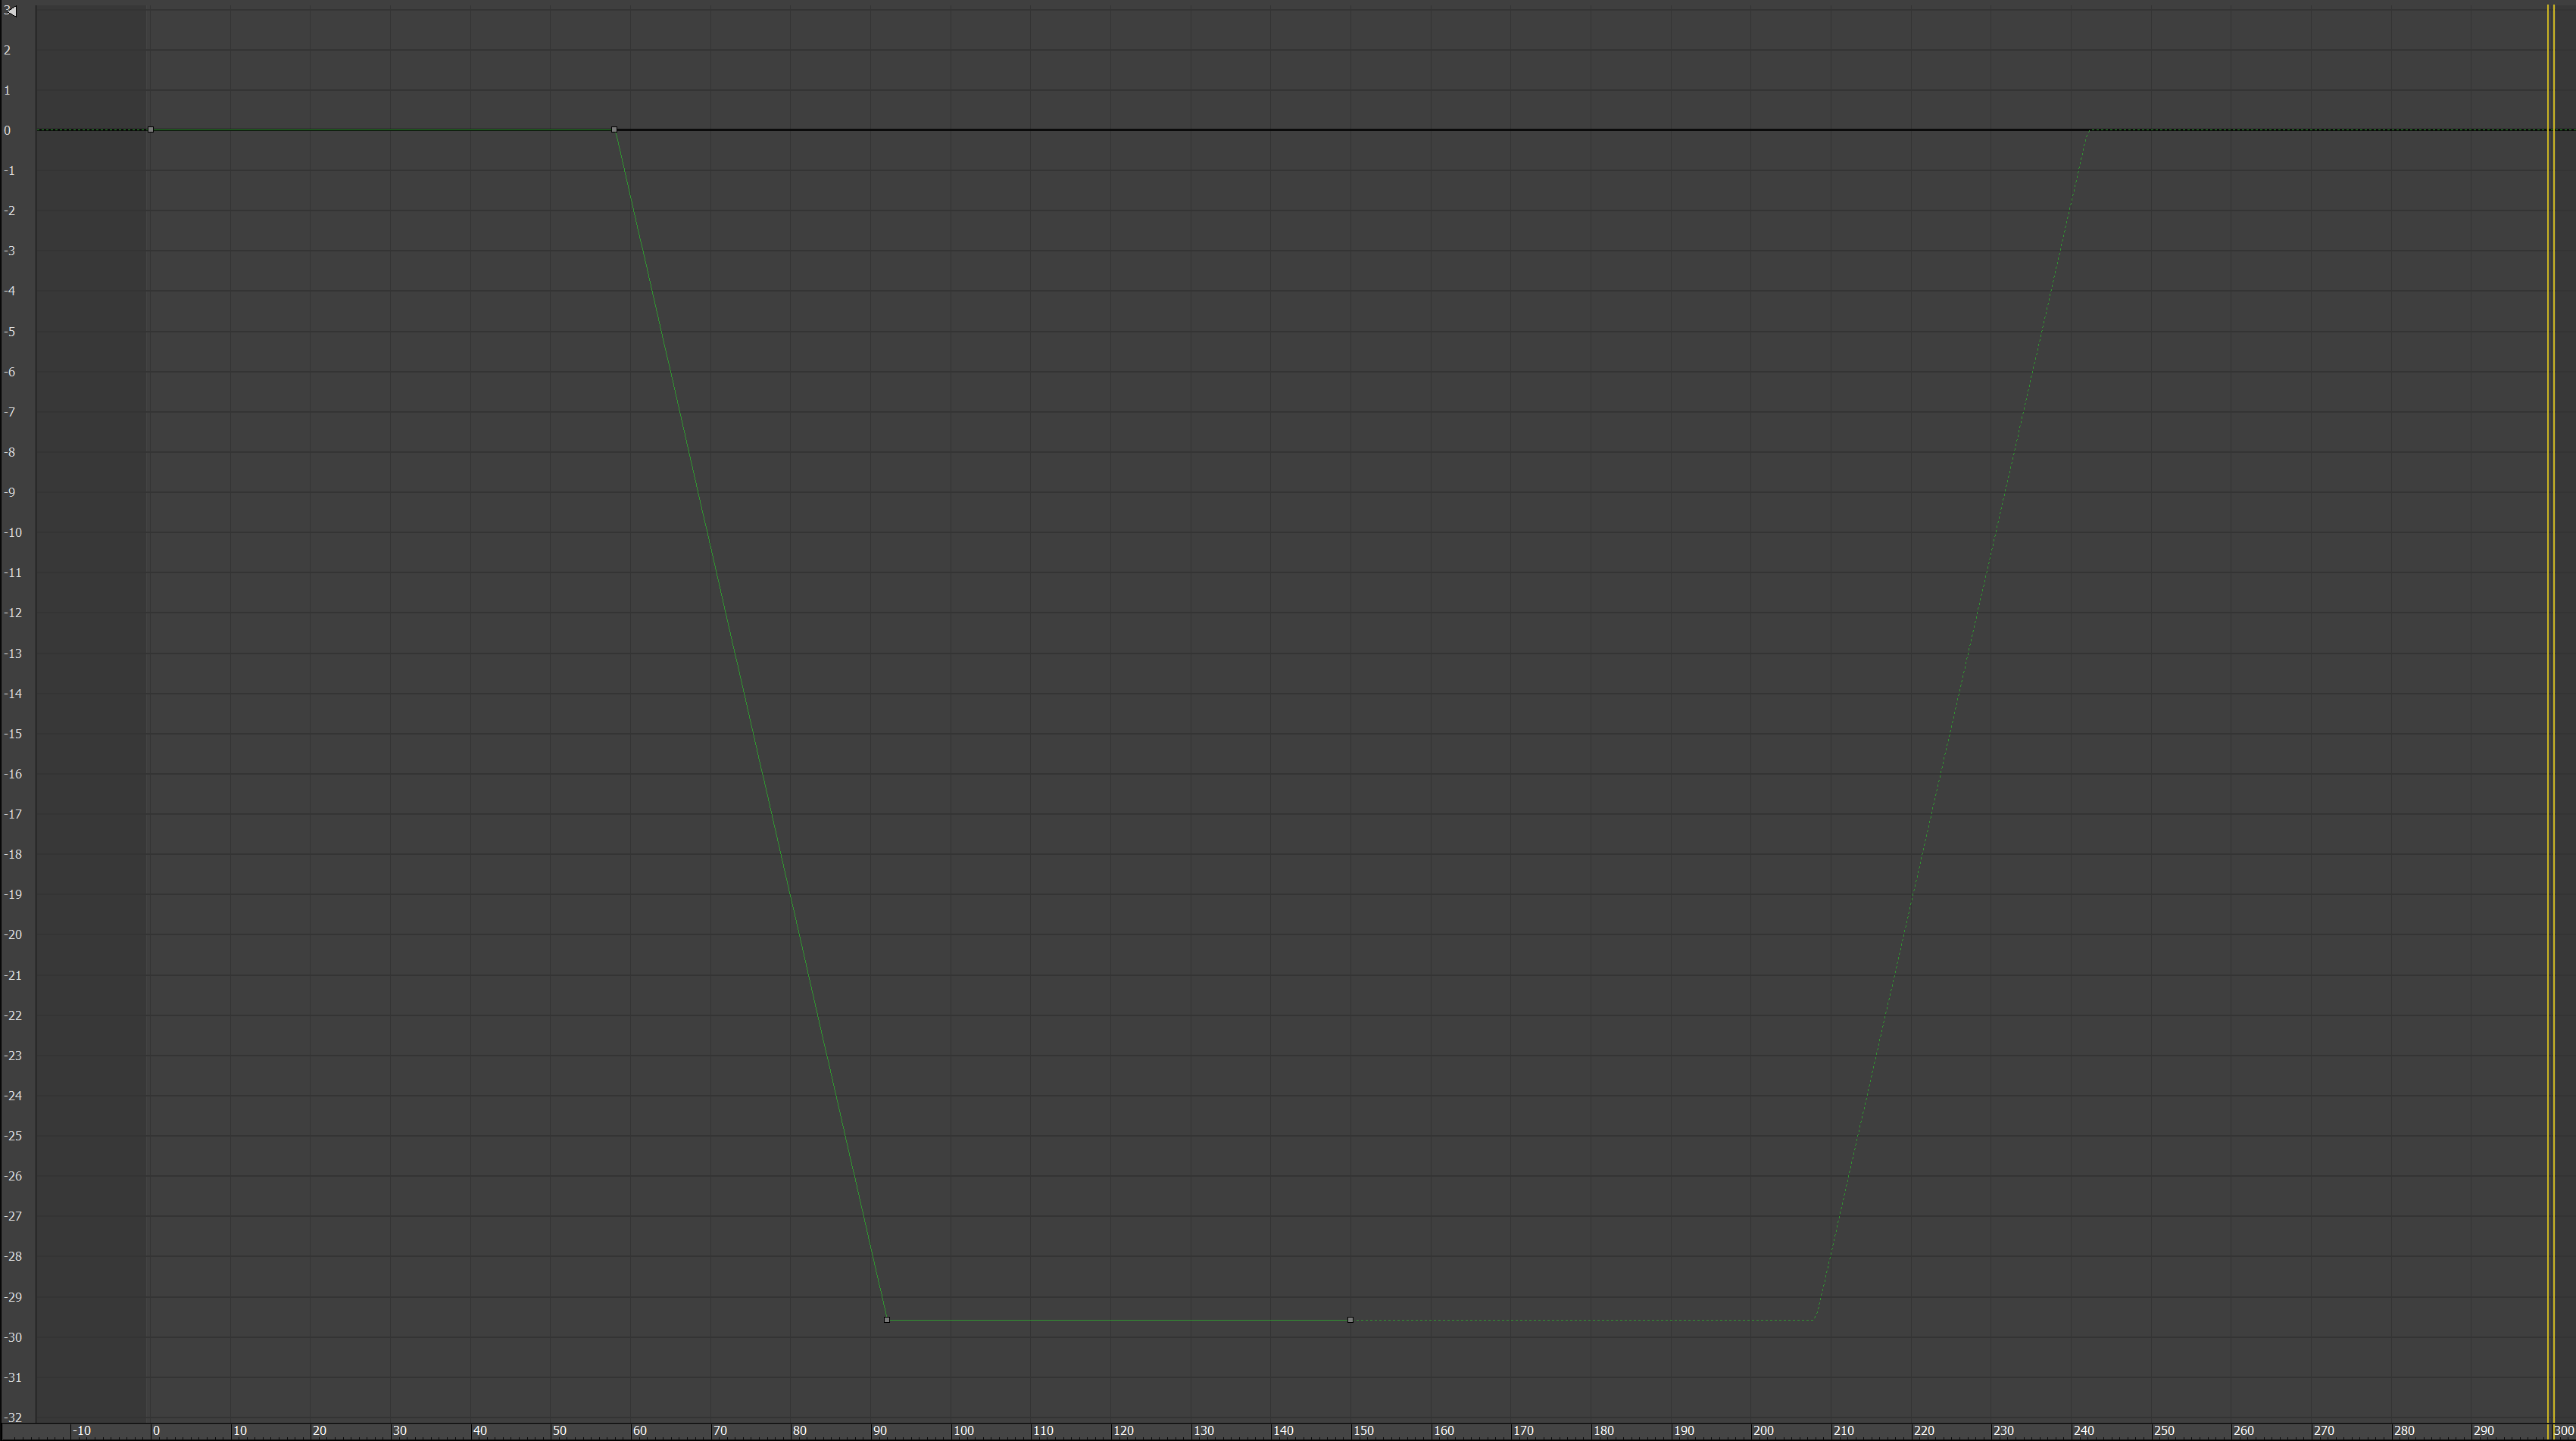
\includegraphics[width=0.7\textwidth]{imagenes/curvas finales/DPL.png}
   \caption{Curva, junto a su inversa, del \textit{Dummy} de la pelota de la izquierda.}
\end{figure}

\begin{figure}[H]
   \centering
   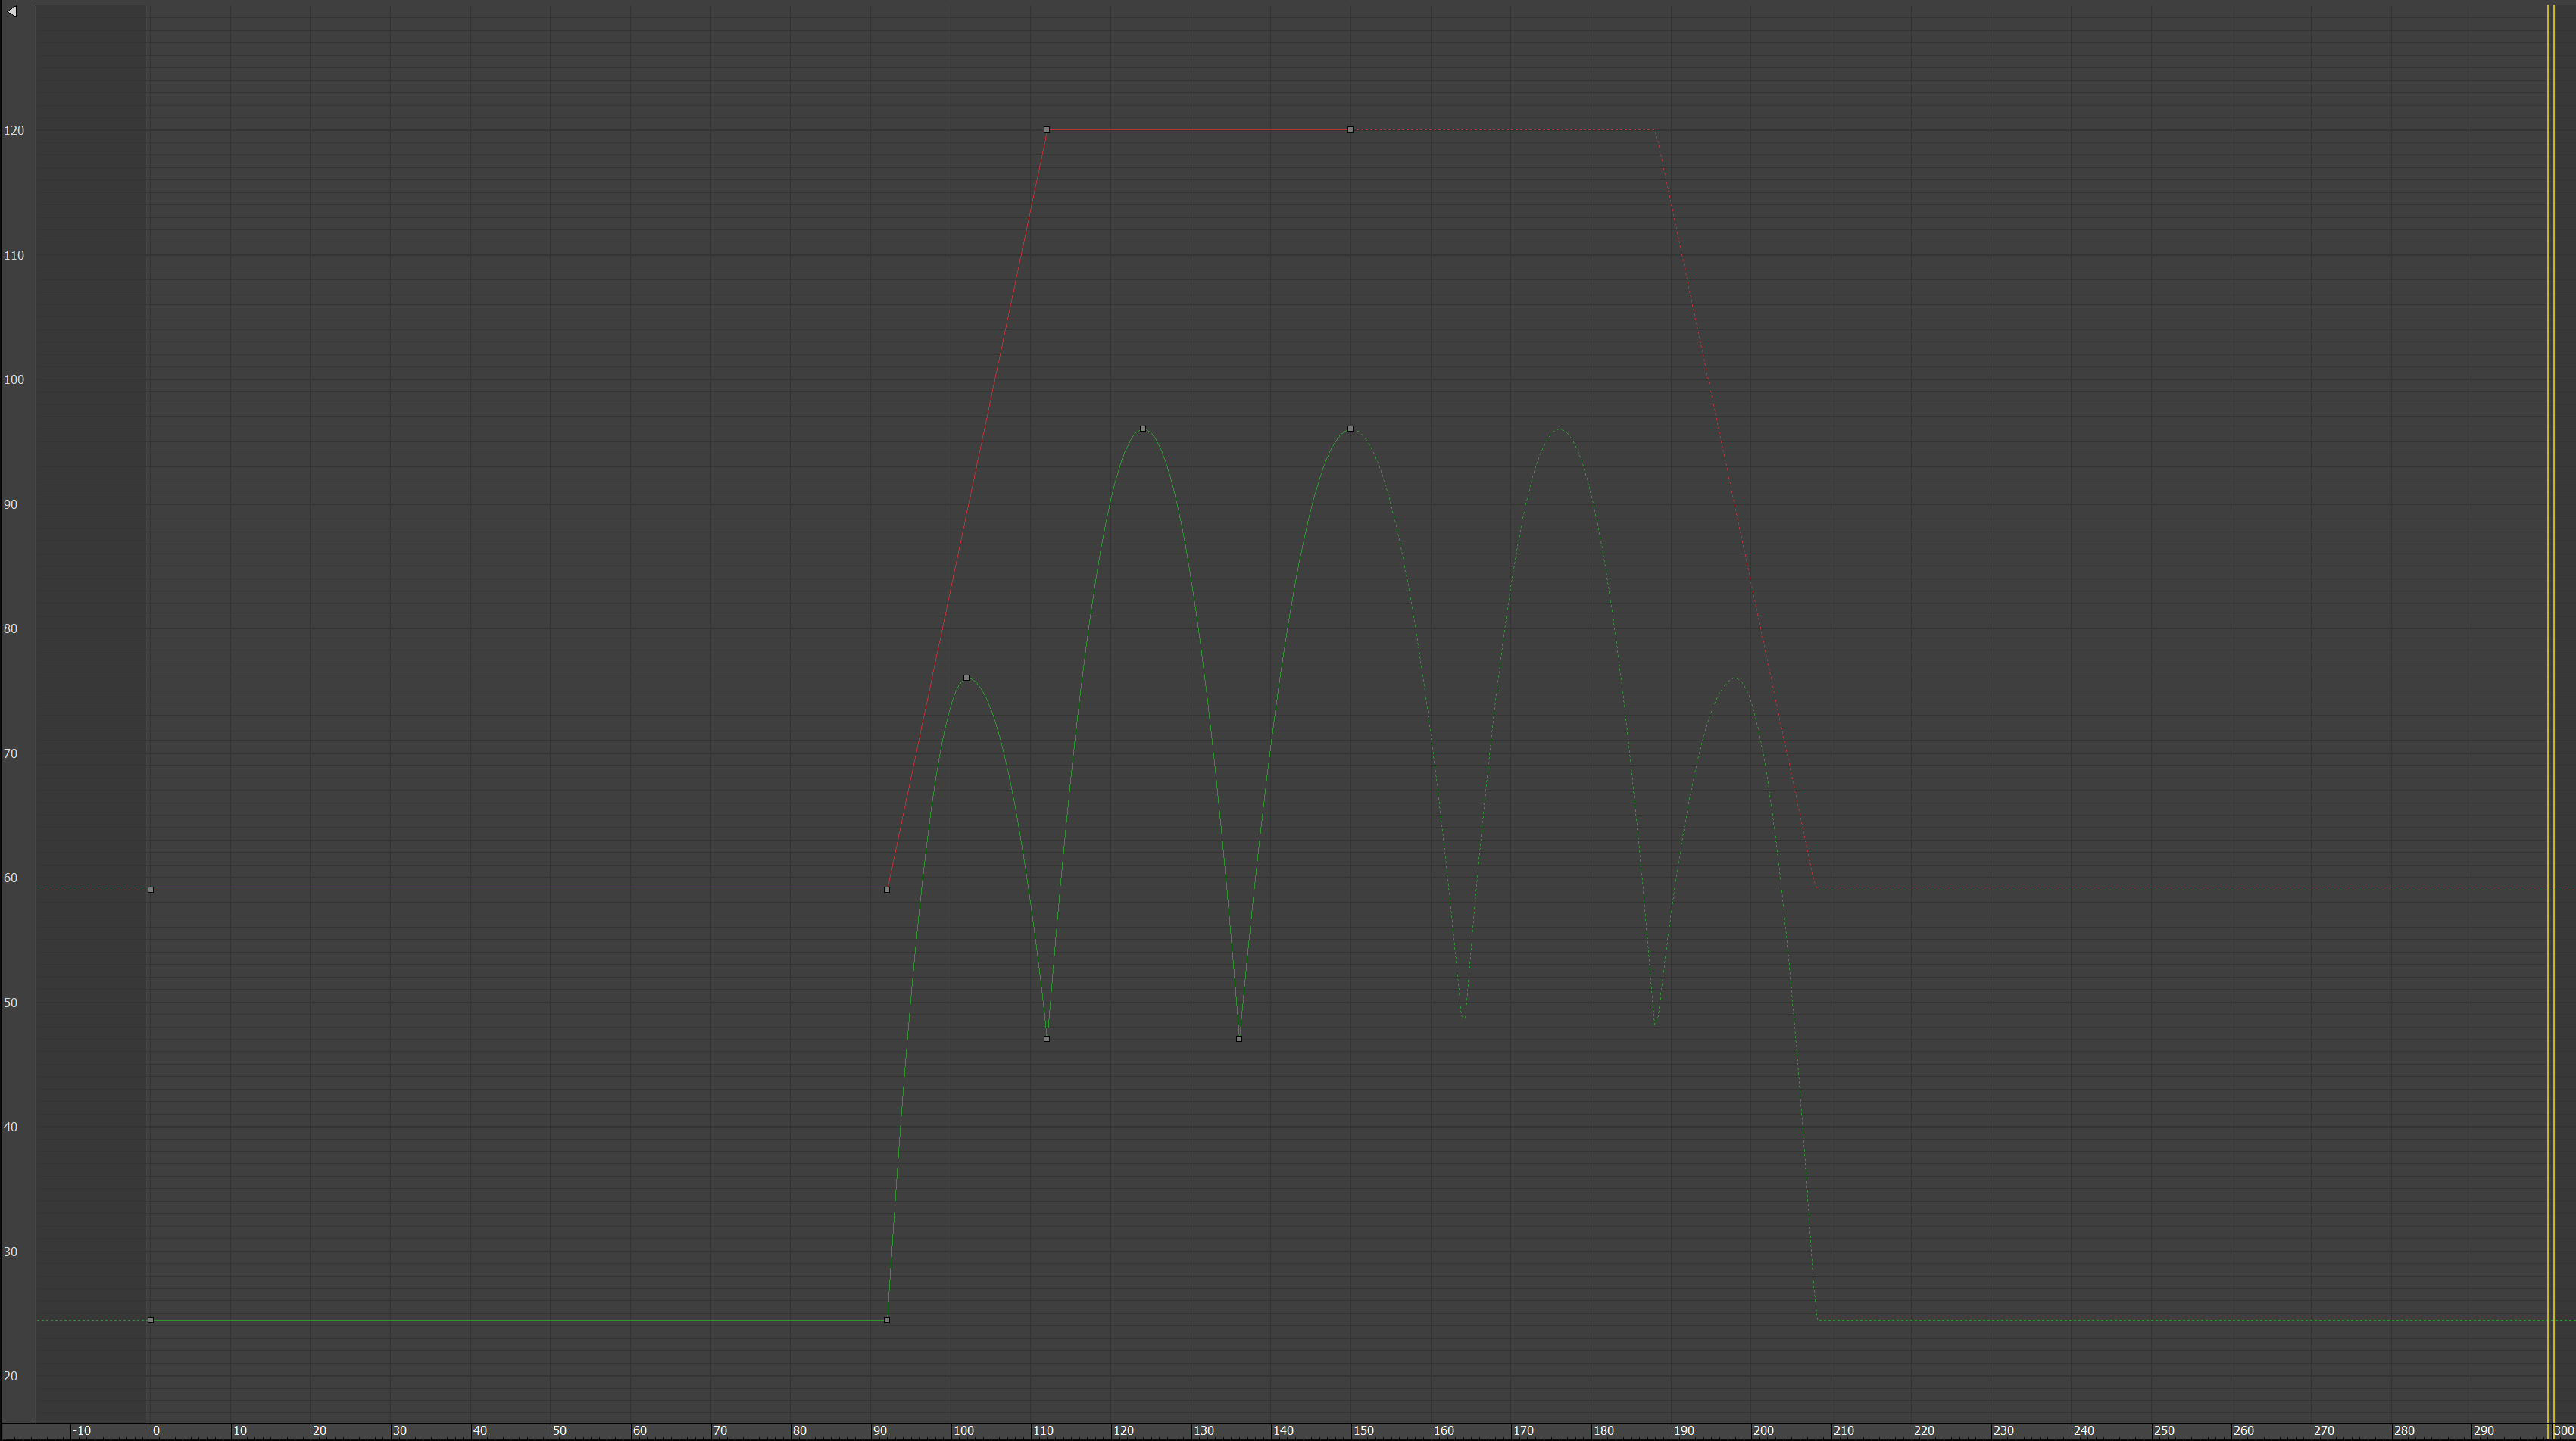
\includegraphics[width=0.7\textwidth]{imagenes/curvas finales/PR.png}
   \caption{Curva, junto a su inversa, de la pelota de la derecha.}
\end{figure}

\begin{figure}[H]
   \centering
   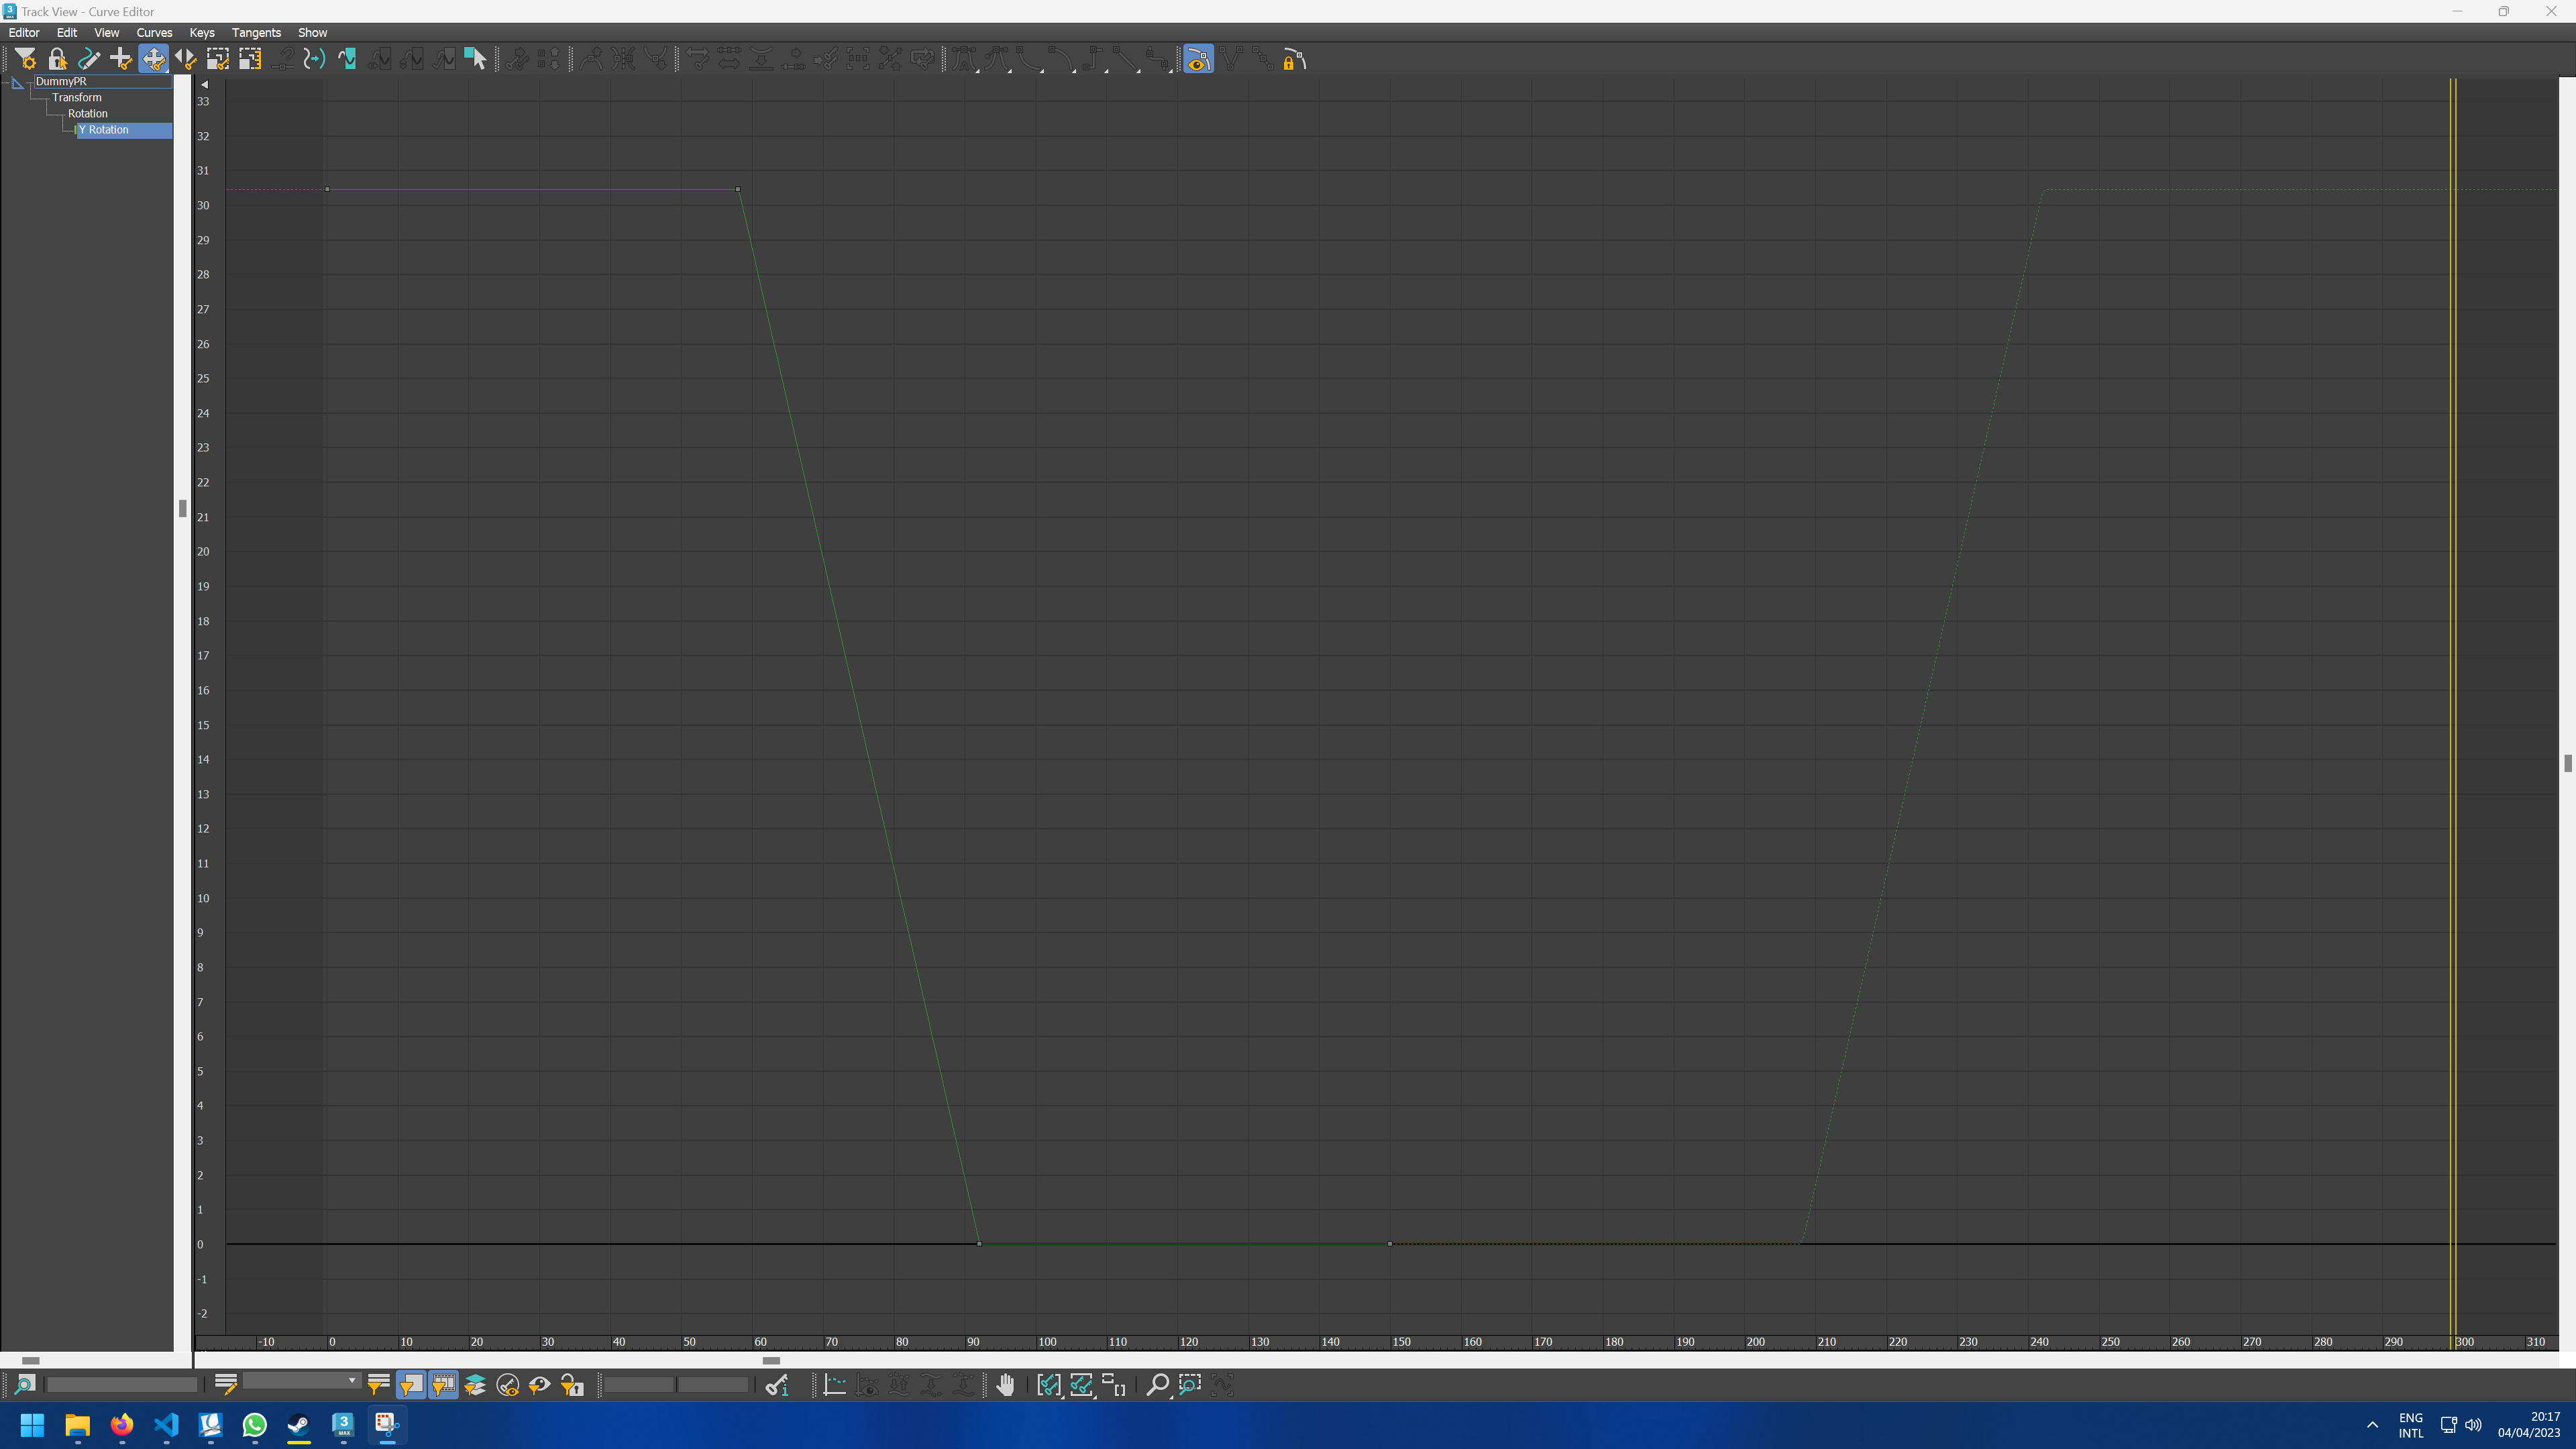
\includegraphics[width=0.7\textwidth]{imagenes/curvas finales/DPR.png}
   \caption{Curva, junto a su inversa, del \textit{Dummy} de la pelota de la derecha.}
\end{figure}

\begin{figure}[H]
   \centering
   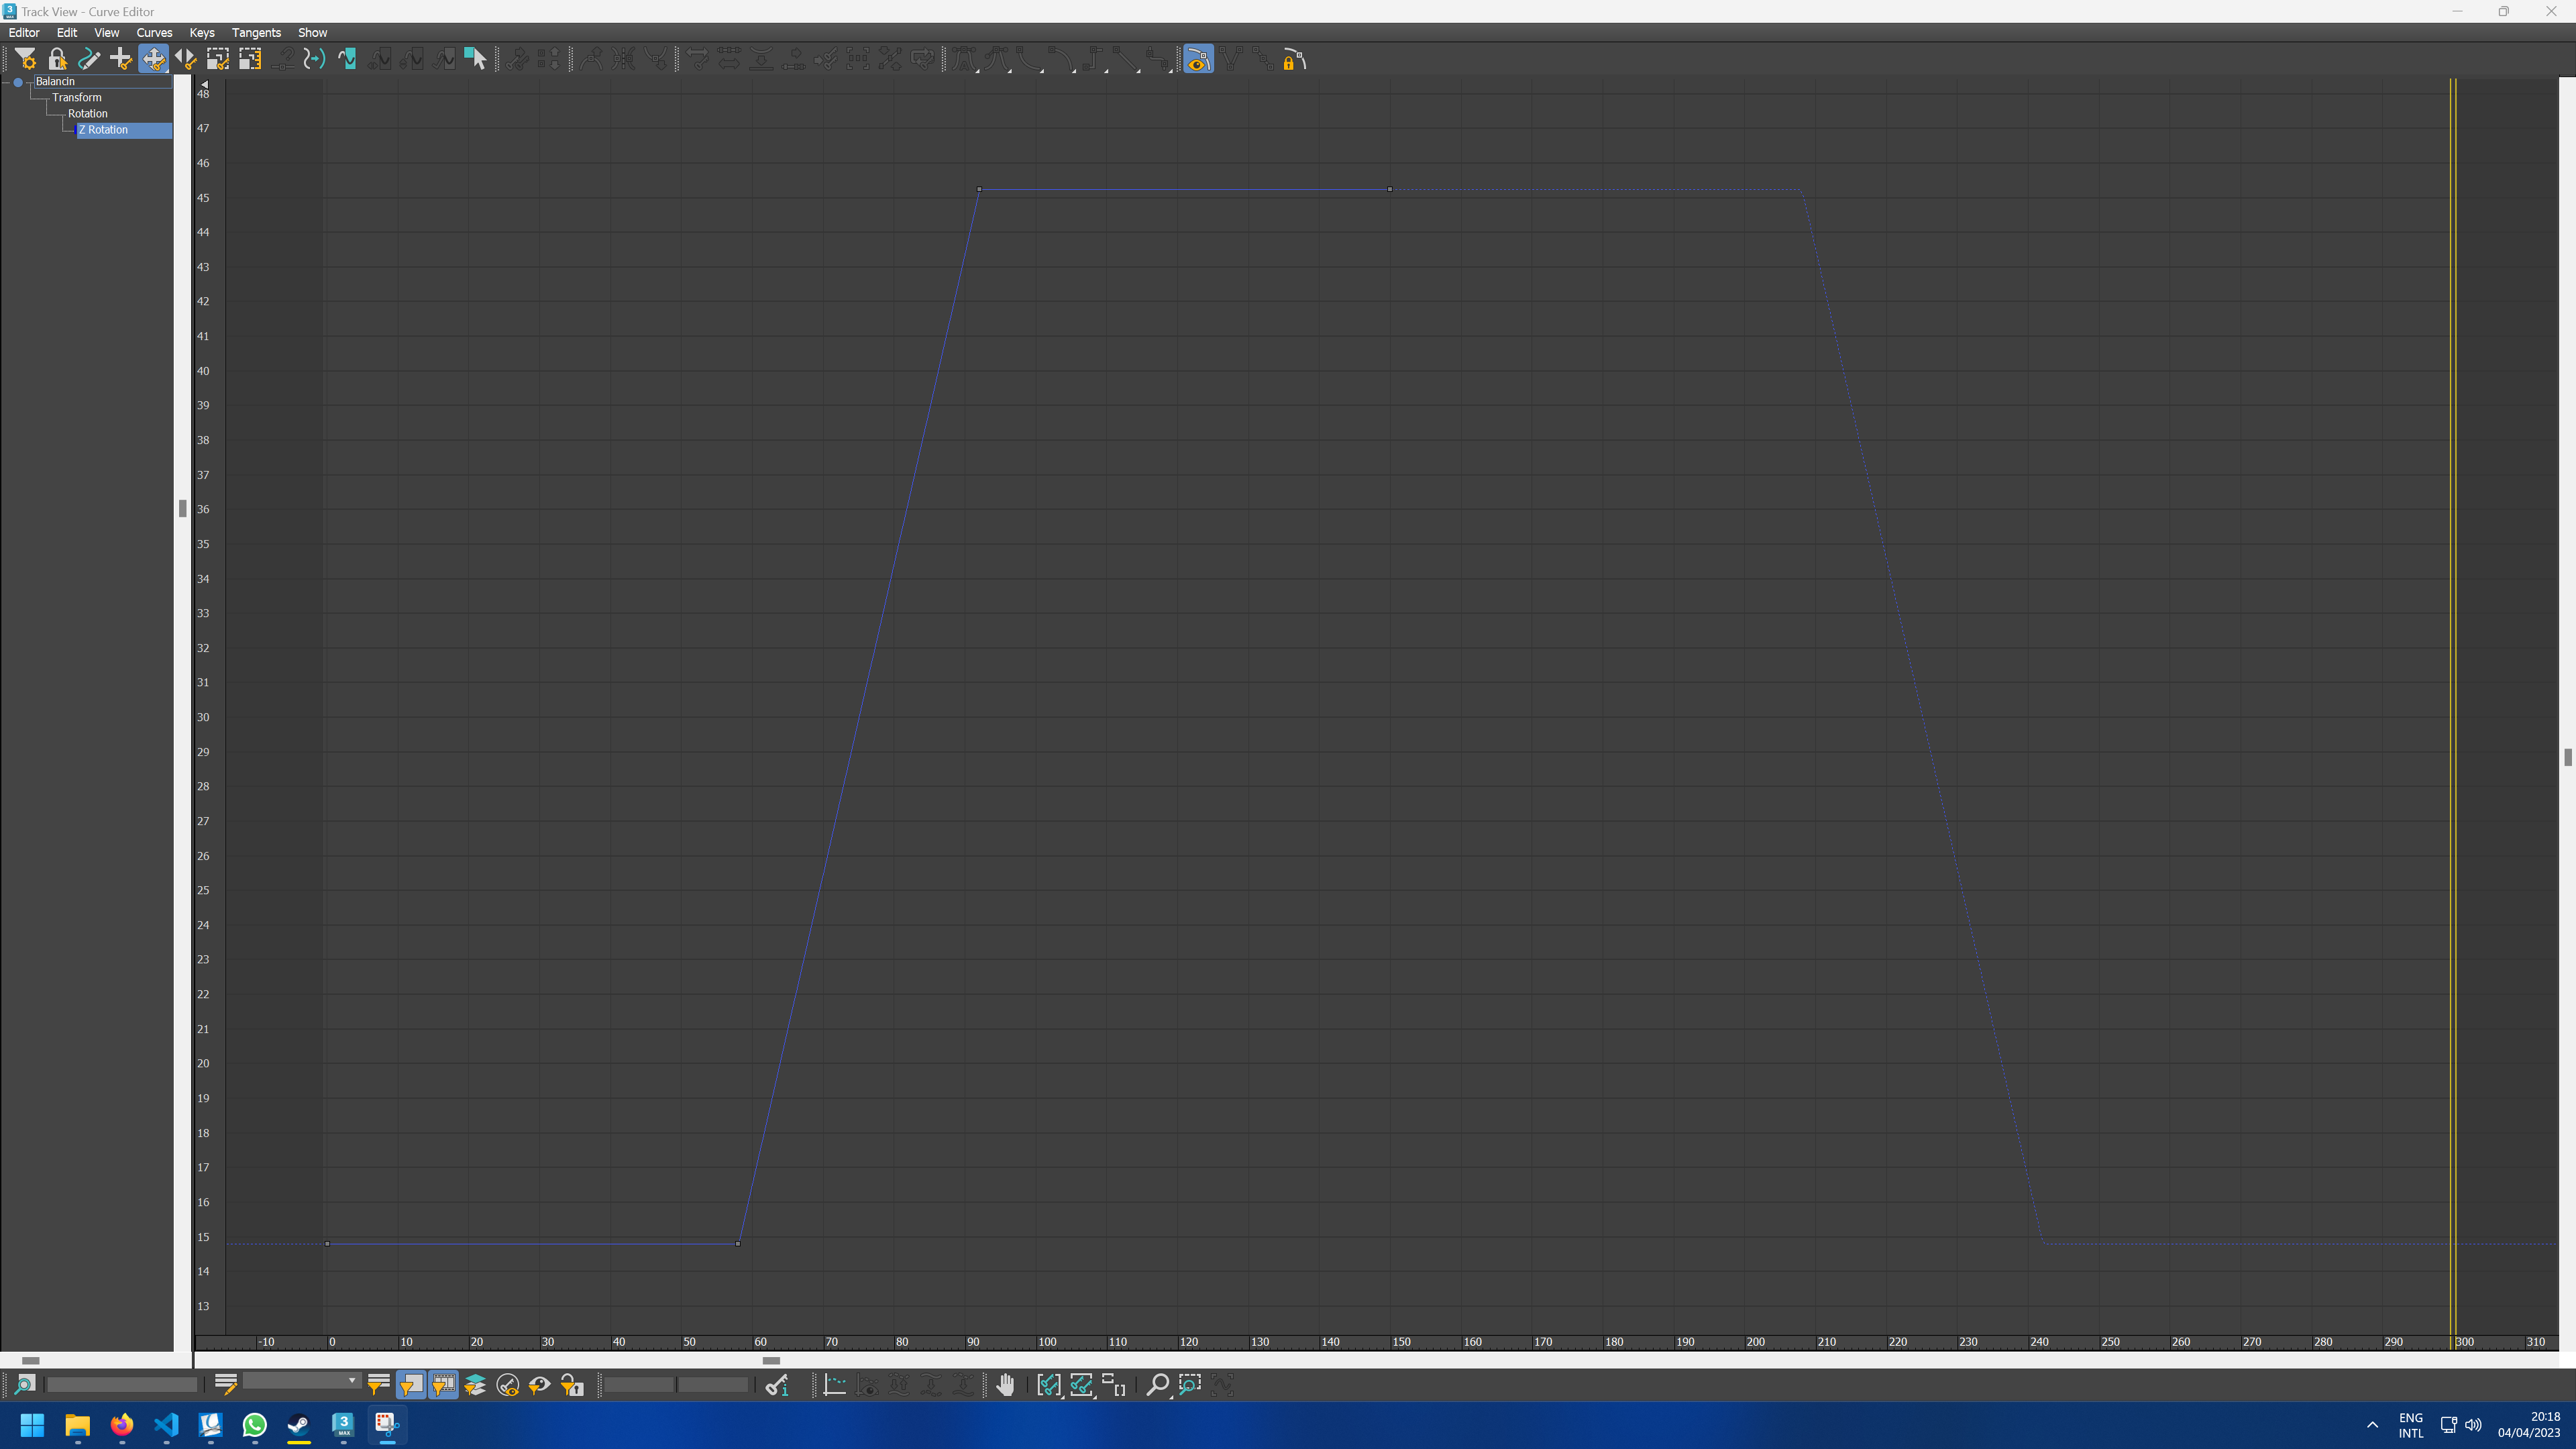
\includegraphics[width=0.7\textwidth]{imagenes/curvas finales/trampolin.png}
   \caption{Curva, junto a su inversa, del trampolín.}
\end{figure}

\begin{figure}[H]
   \centering
   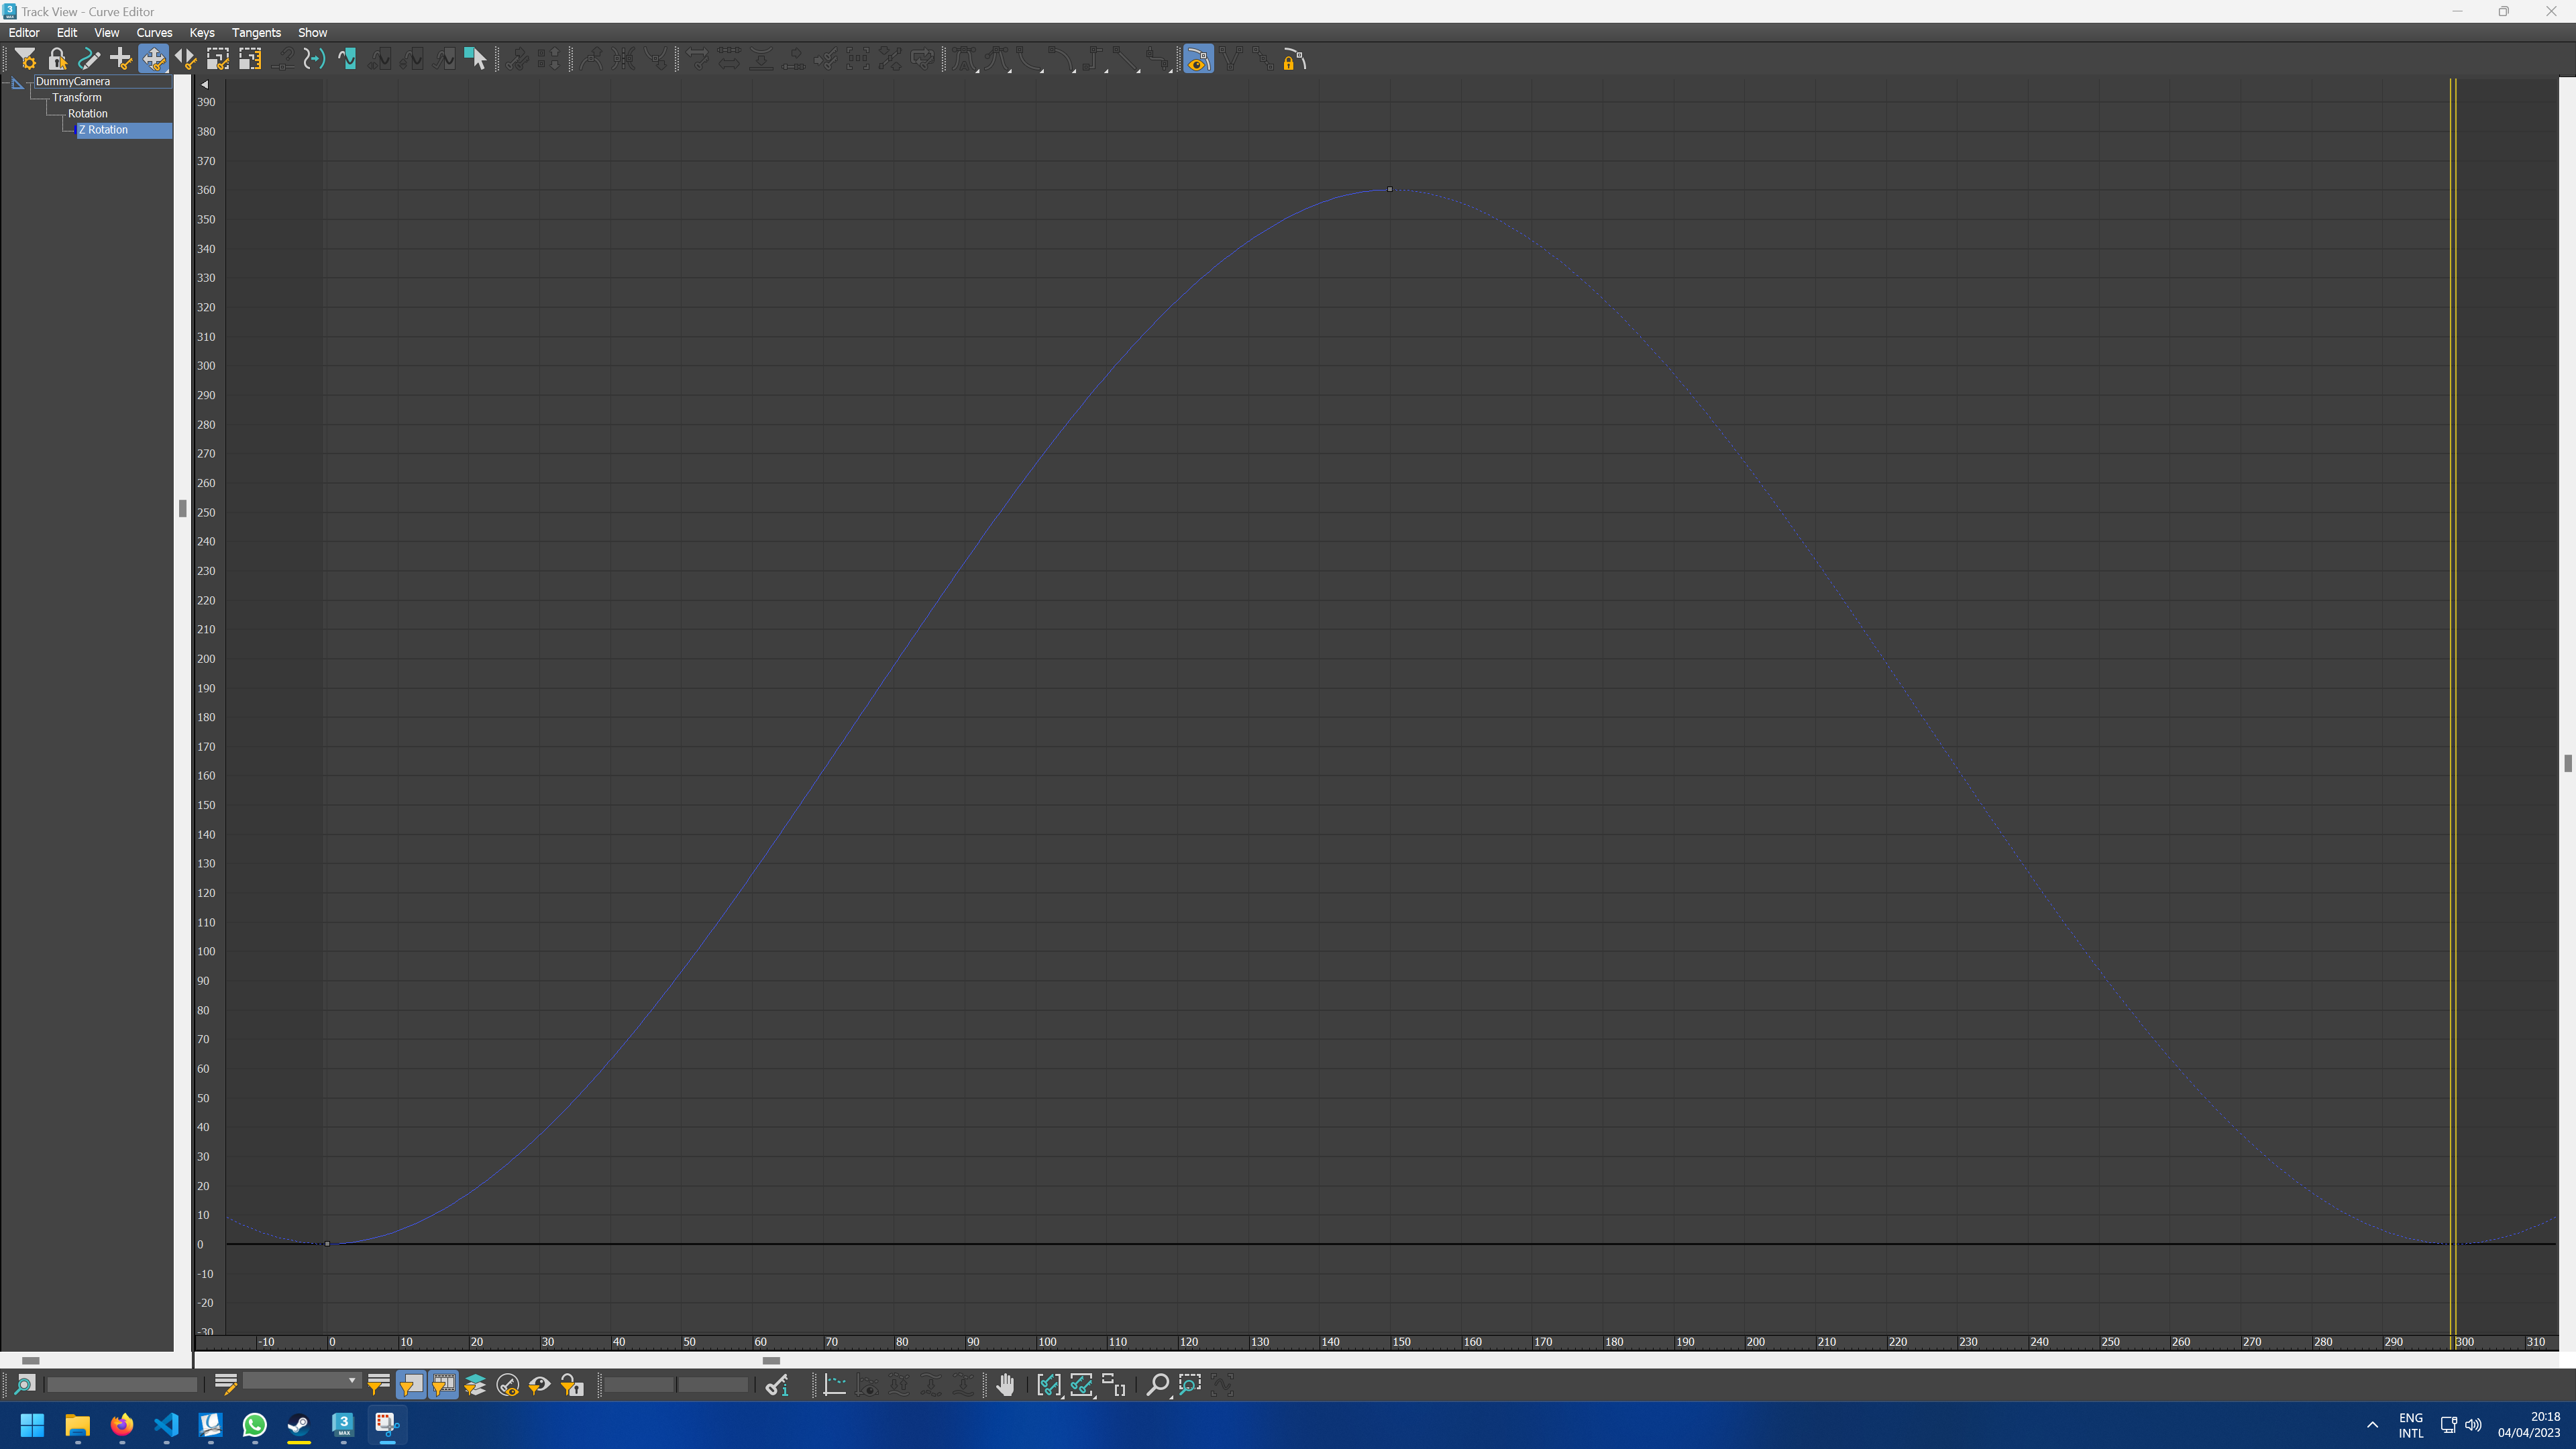
\includegraphics[width=0.7\textwidth]{imagenes/curvas finales/DCamara.png}
   \caption{Curva, junto a su inversa, del \textit{Dummy} utilizado en la cámara.}
\end{figure}

\begin{figure}[H]
   \centering
   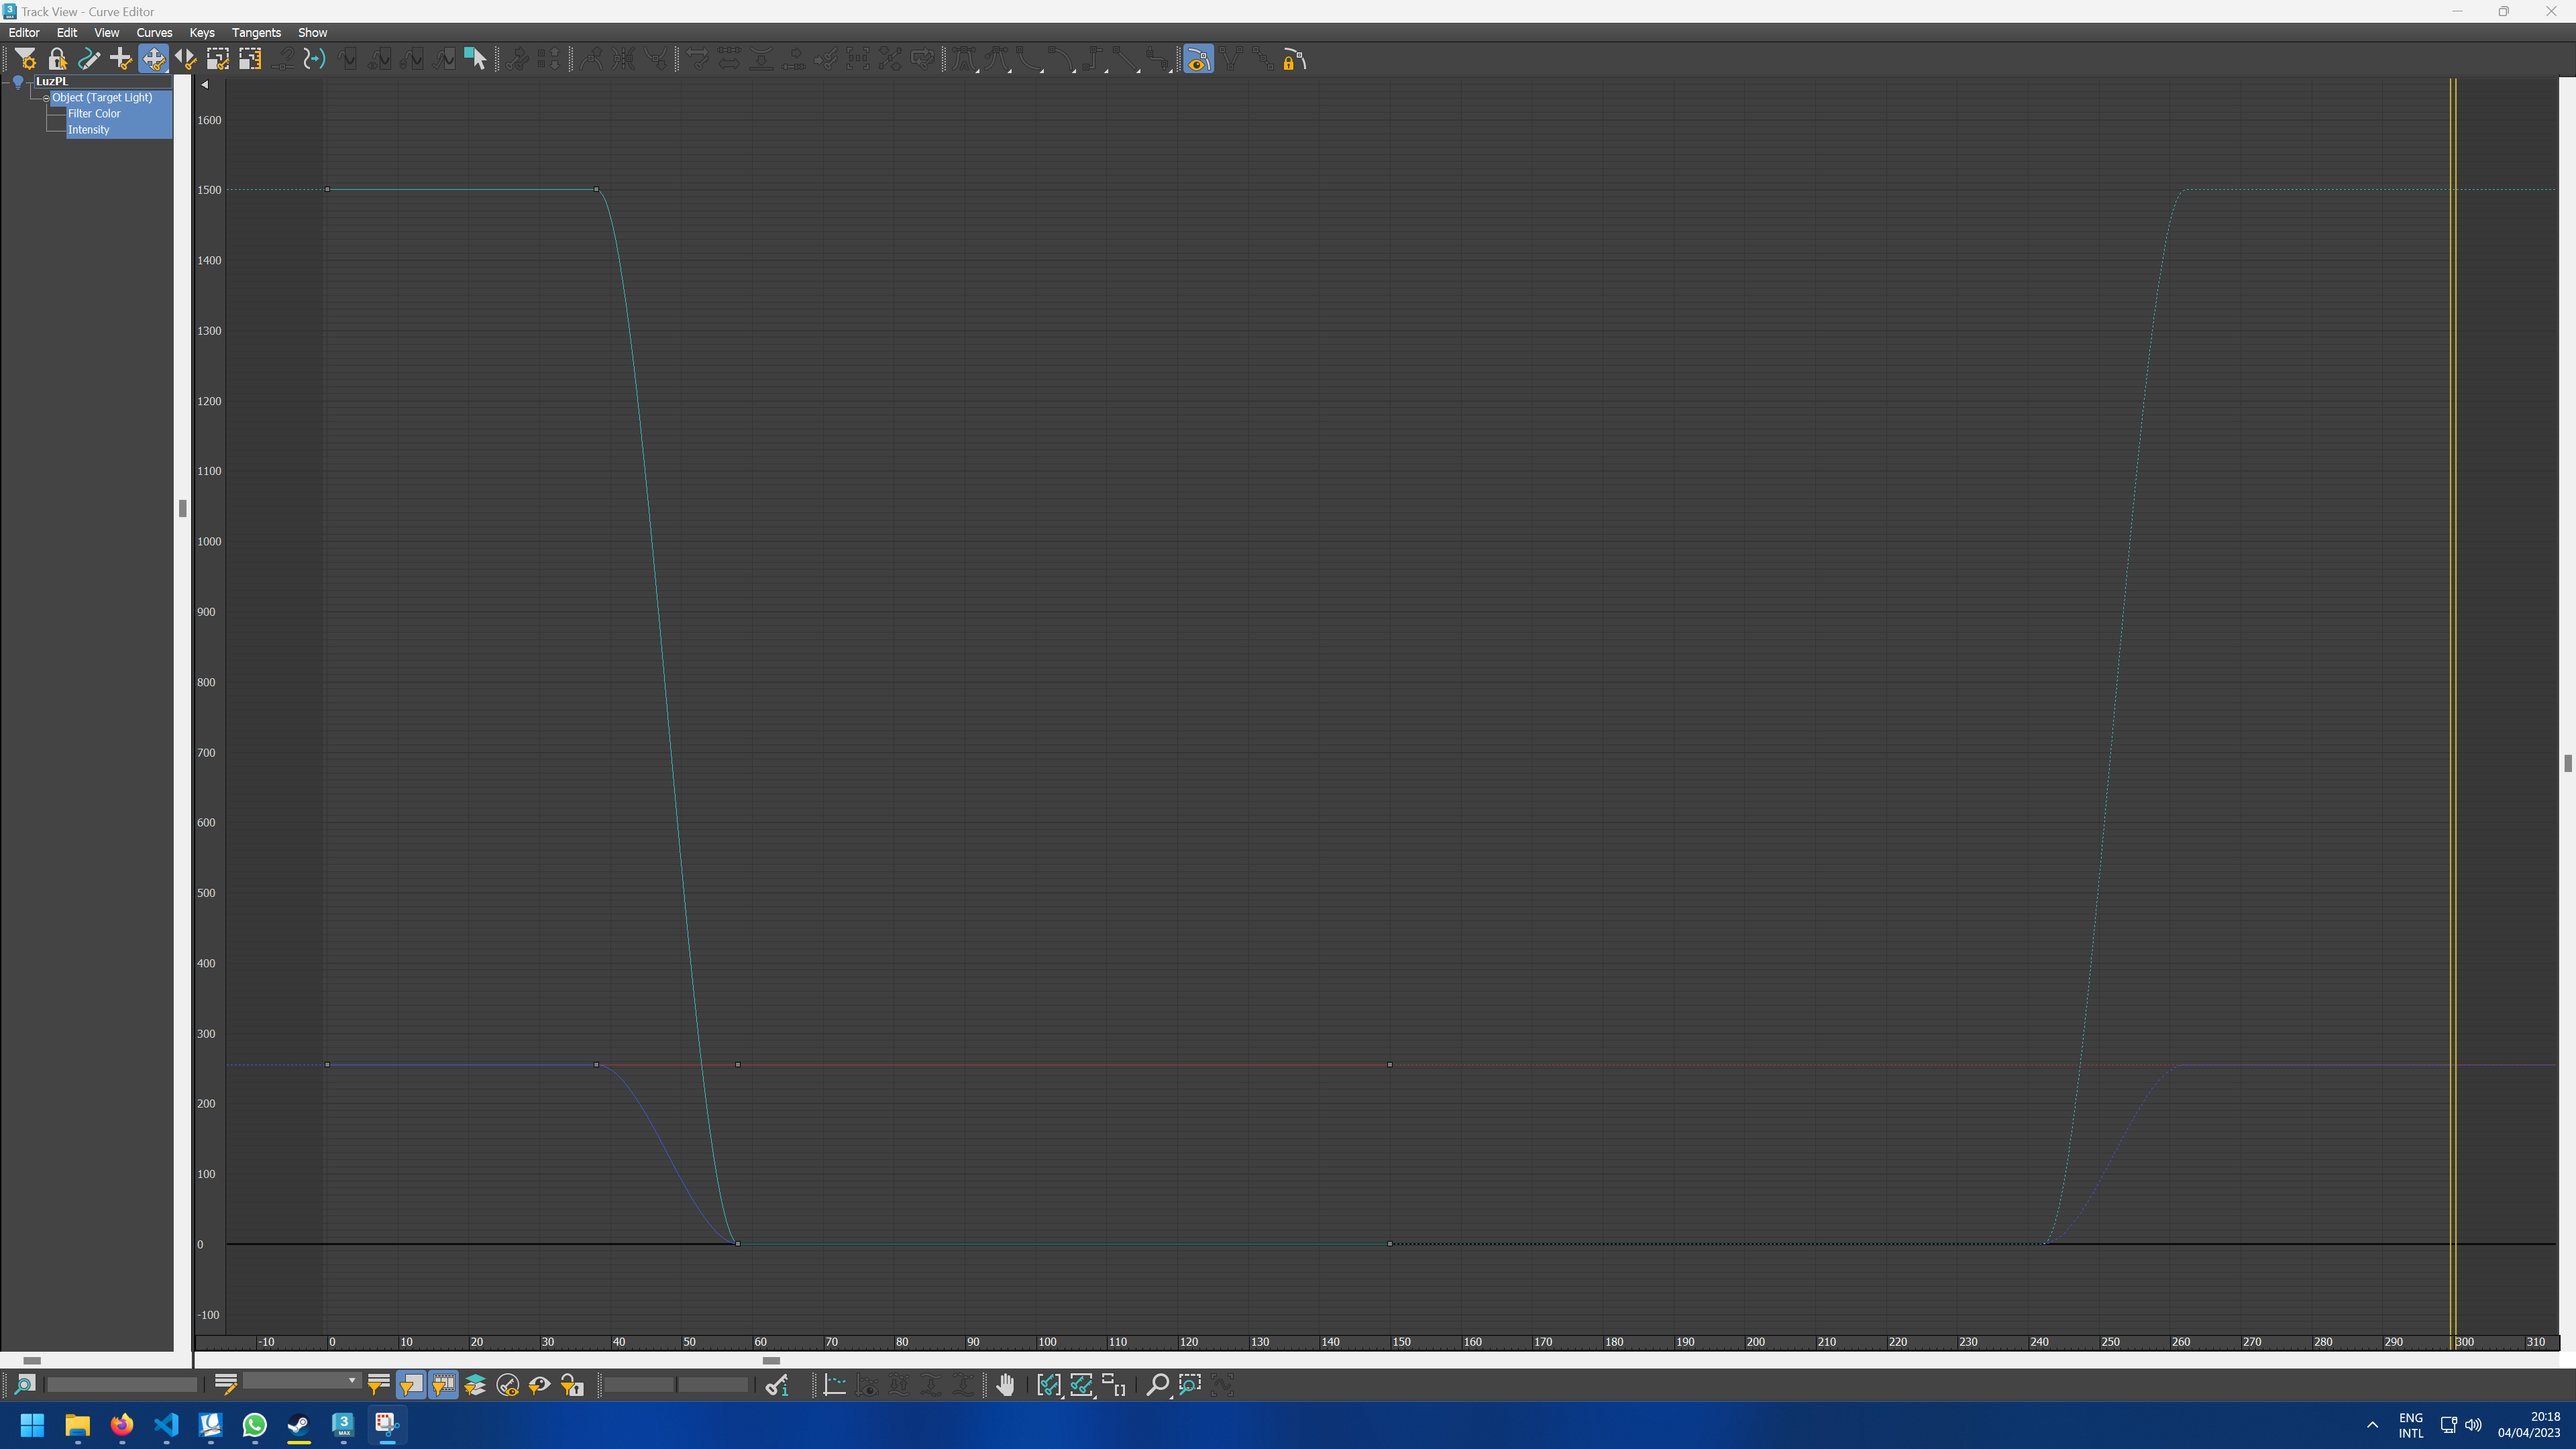
\includegraphics[width=0.7\textwidth]{imagenes/curvas finales/LL.png}
   \caption{Curva, junto a su inversa, de la luz de la izquierda.}
\end{figure}

\begin{figure}[H]
   \centering
   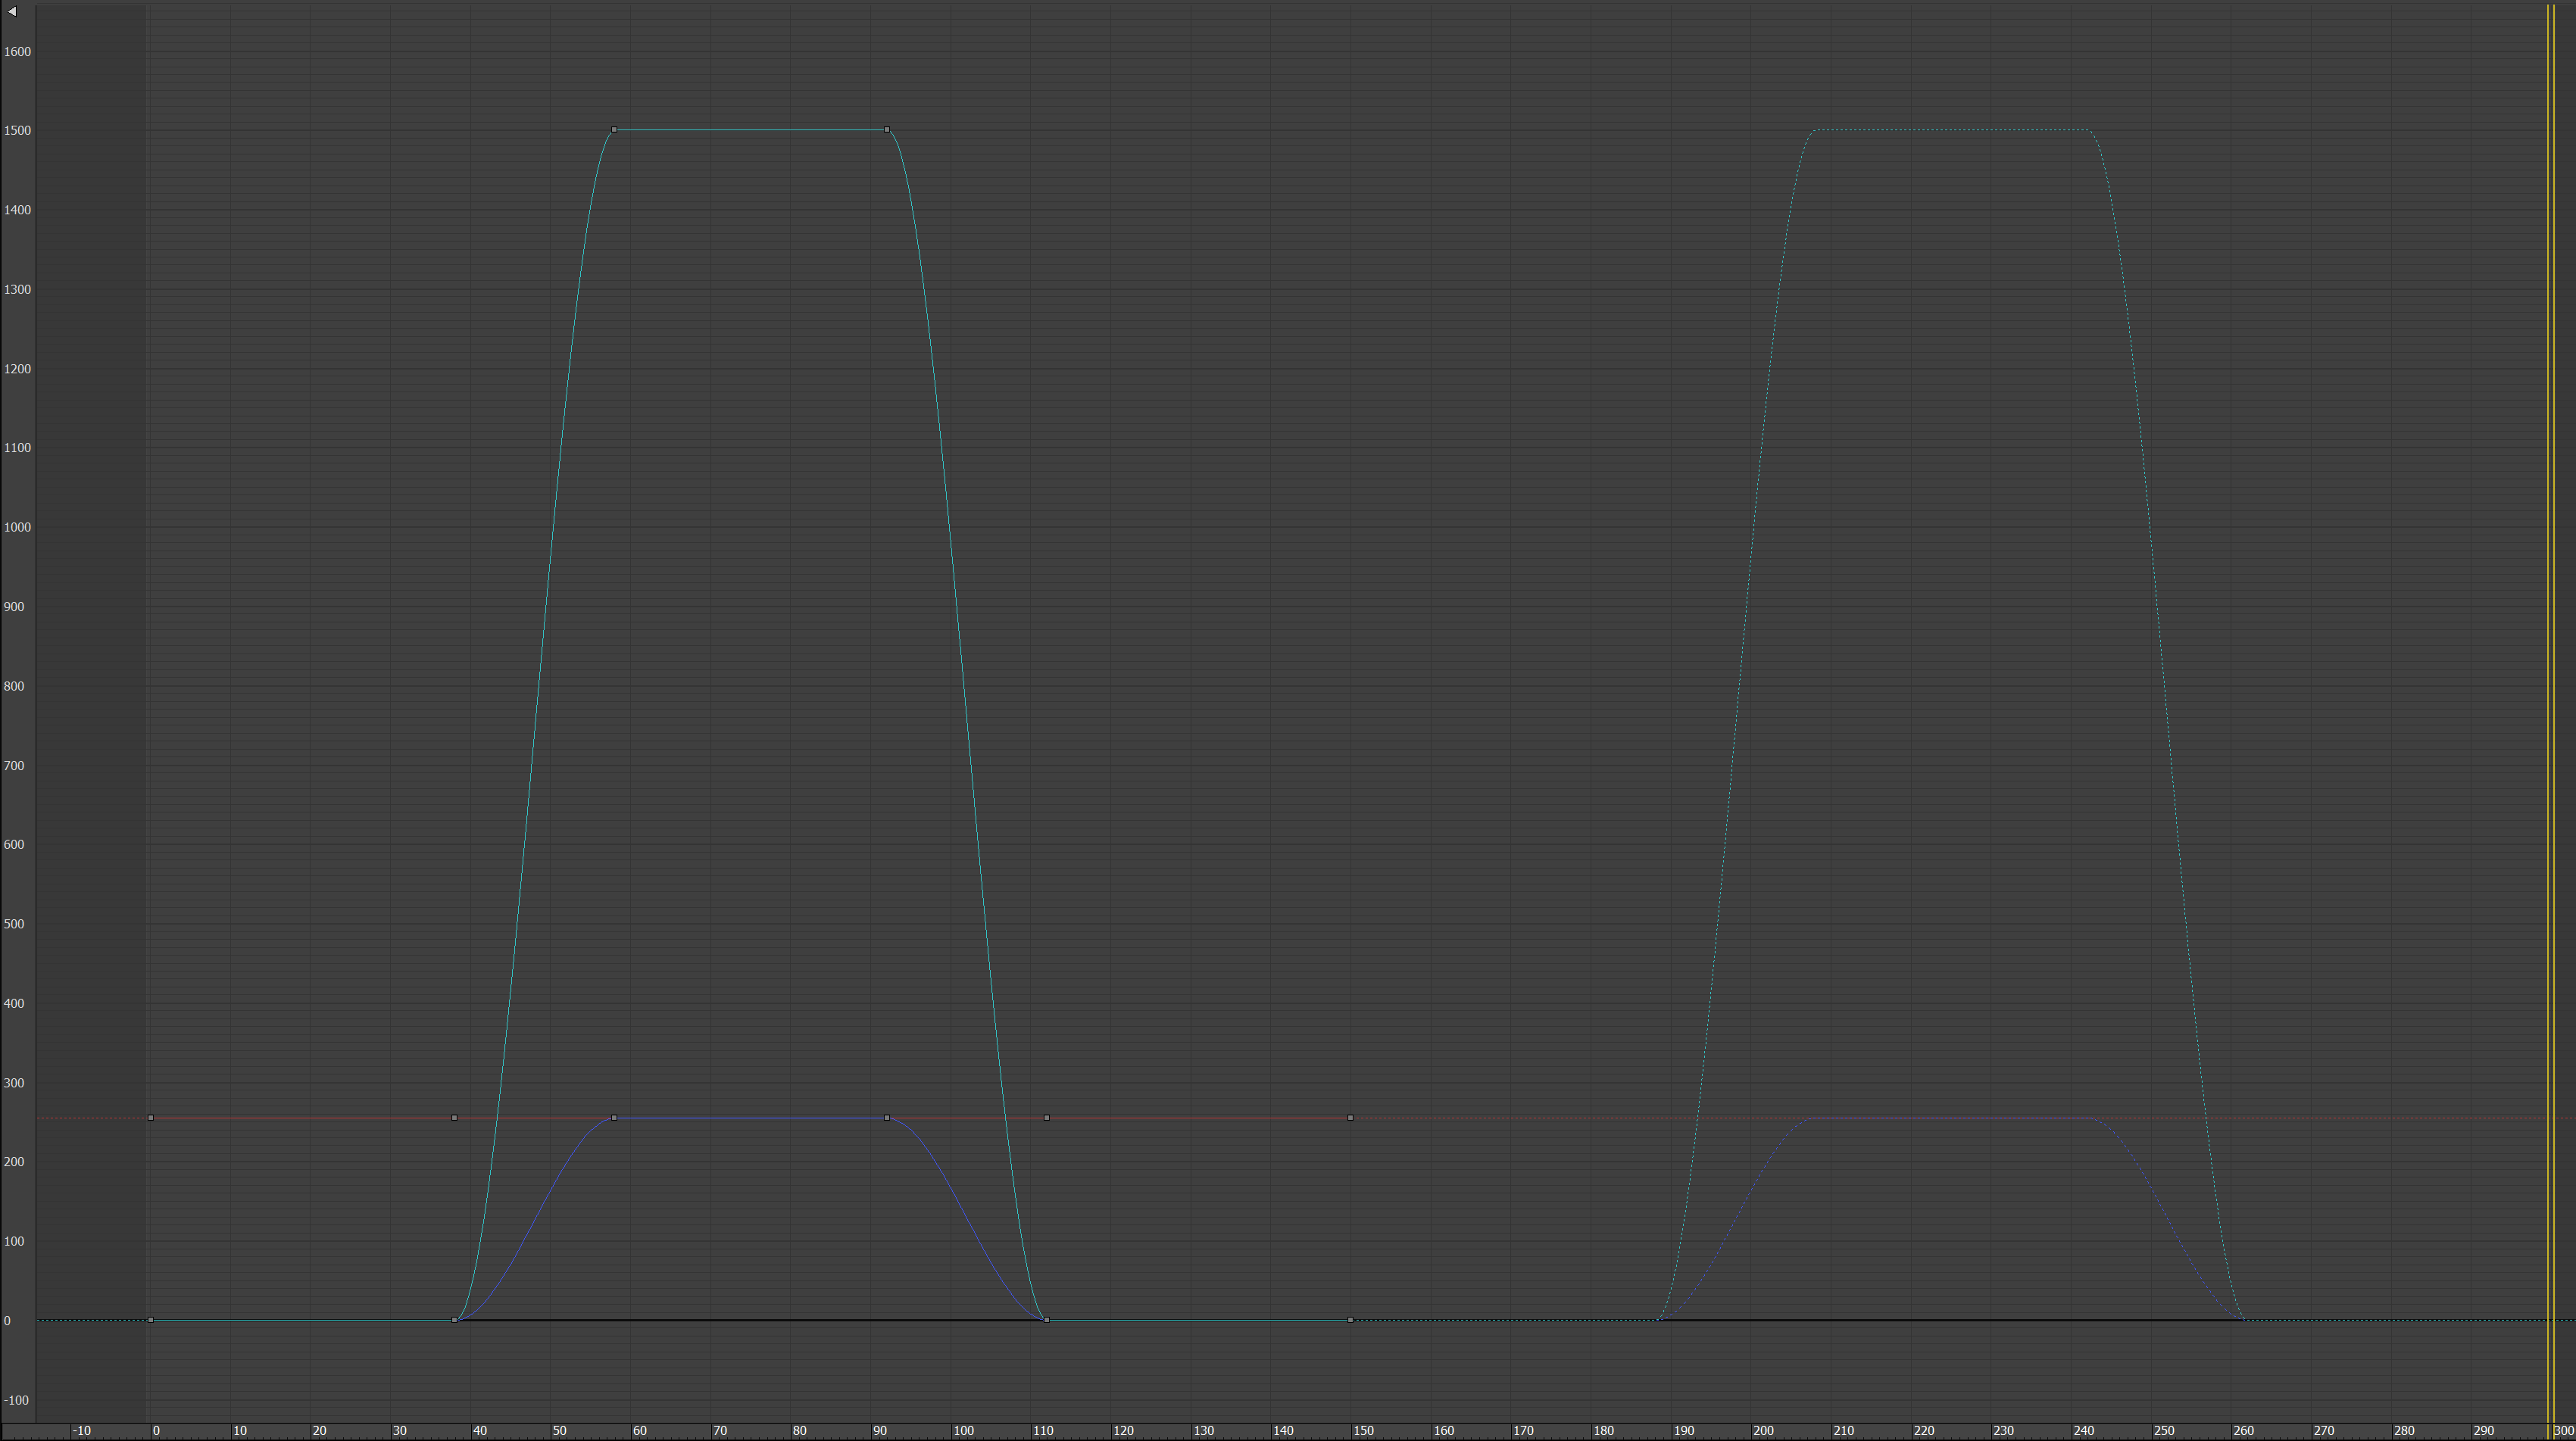
\includegraphics[width=0.7\textwidth]{imagenes/curvas finales/LC.png}
   \caption{Curva, junto a su inversa, de la luz del centro de la escena.}
\end{figure}

\begin{figure}[H]
   \centering
   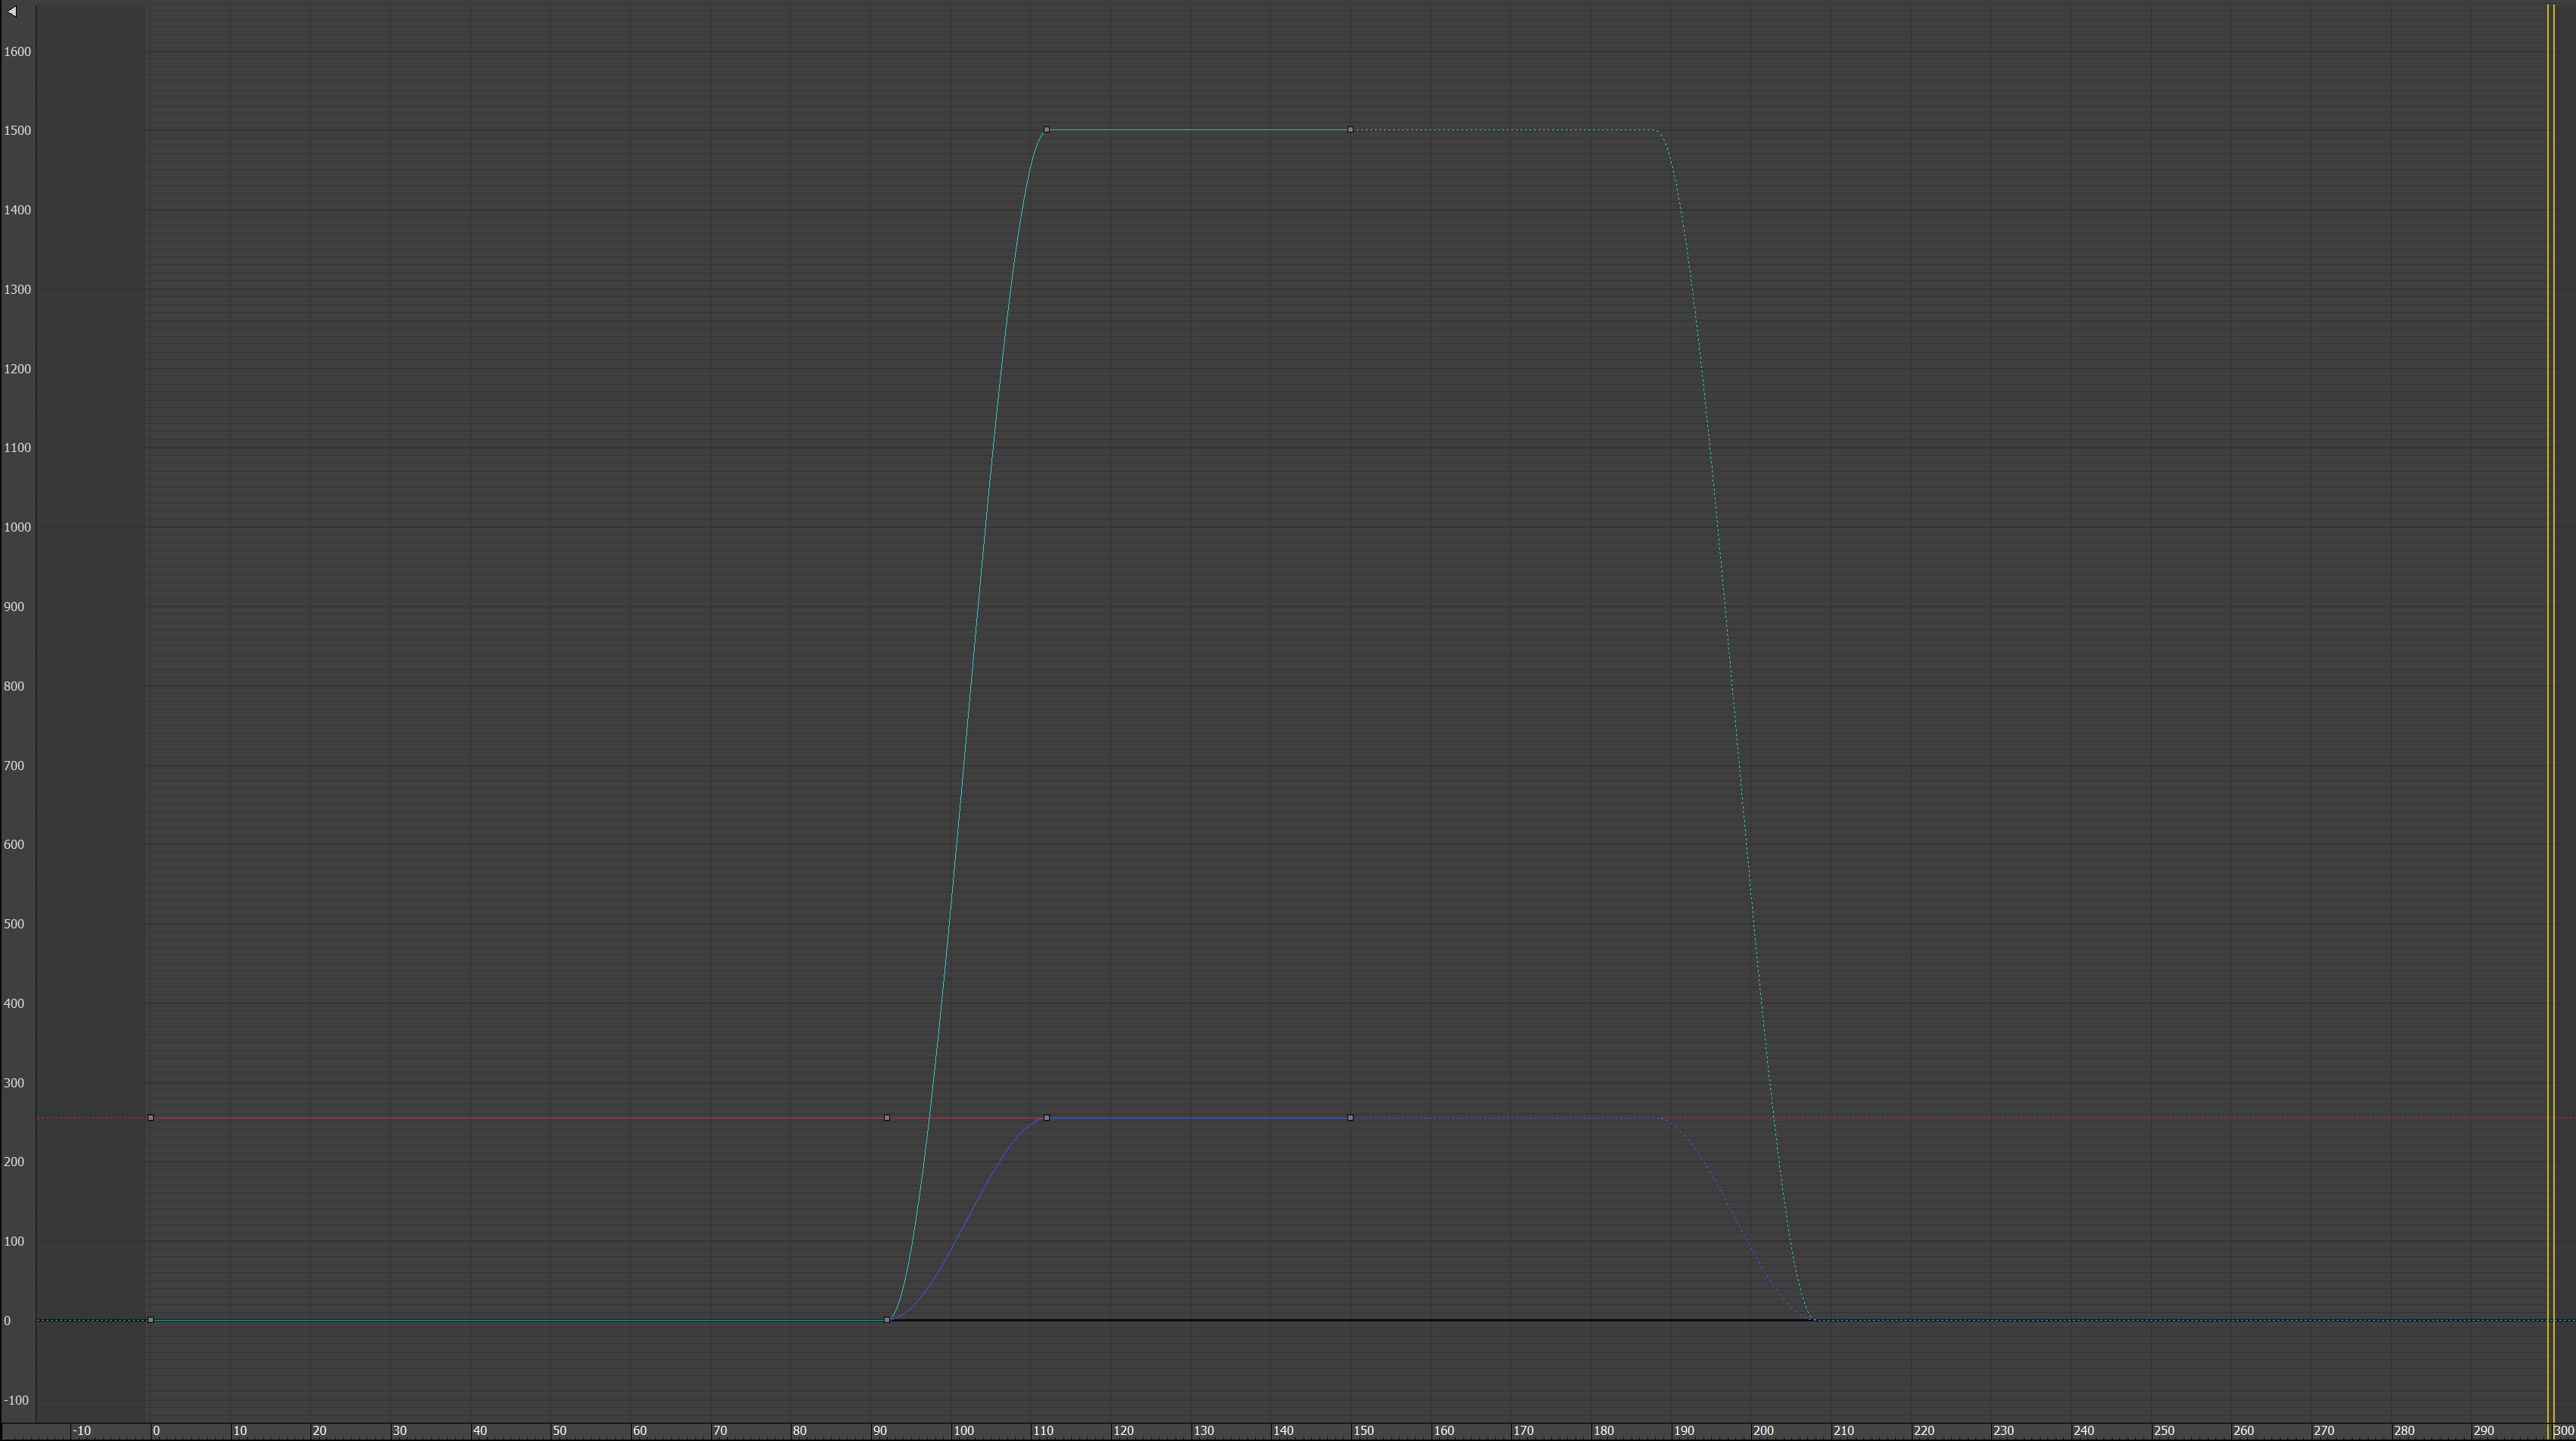
\includegraphics[width=0.7\textwidth]{imagenes/curvas finales/LR.png}
   \caption{Curva, junto a su inversa, de la luz de la derecha.}
\end{figure}

De nuevo, puede parecer que los \textit{keyframes} de algunos objetos en los instantes 0 o 150 sean innecesarios, pero si no se pusieran la animación inversa comenzaría antes de tiempo o incorrectamente.

\newpage